%%
%% licence       kaneton licence
%%
%% project       kaneton
%%
%% file          /home/buckman/kaneton/view/books/kaneton/core.tex
%%
%% created       matthieu bucchianeri   [mon jan 30 17:33:29 2006]
%% updated       matthieu bucchianeri   [wed feb  7 22:17:27 2007]
%%

%
% core
%

\chapter{Core}

In this chapter we will describe the kaneton core design and implementation.

We will precisly describe the core's managers taking care of specifying the
interface it provides.

\newpage

%
% text
%

The kaneton microkernel is composed of managers. Each manager provides
an interface to manipulate a special kaneton object or something else.

%
% id manager
%

\section{id manager}

The \textbf{id manager} provides an interface to manipulate the
kaneton identifiers.

The \textbf{id object} \textit{o\_id} is used to generate unique
- in its own name space - identifiers \textit{t\_id}.

In the current kaneton implementation, identifiers only consist in 64-bit
integers. Therefore, the id manager does not take care of identifiers
recycling. Nevertheless, the id manager interface was designed to permit
identifiers recycling.

Note that the id manager is the very first manager to be initialized. Then
the whole core will use it to generate identifiers for the other kaneton
objects.

%
% interface
%

\subsubsection{Interface}

\function{id\_show}{(o\_id* \argument{o})}
	 {
	   This function just displays the state of the id object
	   \argument{o}.
	 }

\function{id\_clone}{(o\_id* \argument{o},
                      t\_id \argument{old},
                      t\_id* \argument{new})}
	 {
	   This function duplicates an id object using the \argument{o}
	   identifier object, name space.

	   Note that cloning an identifier means reserving a new one
	   with the same properties.
	 }

\function{id\_reserve}{(o\_id* \argument{o},
                        t\_id* \argument{i})}
	  {
	    This function reserves an identifier \argument{i} using the
	    identifier object \argument{o}.
	  }

\function{id\_release}{(o\_id* \argument{o},
                        t\_id \argument{i})}
	 {
	   This function releases the identifier \argument{i}.
	 }

\function{id\_build}{(o\_id* \argument{o})}
	 {
	   This function initializes an identifier object.
	 }

\function{id\_destroy}{(o\_id* \argument{o})}
	 {
	   This function destroys an identifier object.
	 }

\function{id\_initialize}{(void)}
	 {
	   This function just initializes the id manager.
	 }

\function{id\_clean}{(void)}
	 {
	   This function just cleans the id manager.
	 }

%
% set manager
%

\section{set manager}

The \textbf{set manager} is used to manage the data structures in order
to simplify the other kernel managers. Indeed, every kernel manager
including the task manager, the thread manager, the segment manager etc.
uses the set manager to store the data rather than create and manage data
structures by their own.

More precisly, the set manager is used to store kaneton objects.
As seen earlier, kaneton objects has a first 64-bit field representing
the kaneton object's identifier. Then, the set manager uses this identifier
to retrieve an object in a set.

Notice that to avoid problems, a set must contain objects with unique
identifiers. Indeed, identifier collisions in sets are not permitted.

The set manager manages set objects. A \textbf{set object} \textit{o\_set}
is a kaneton object so is identified by a unique set identifier
\textit{i\_set}.

The set mecanism is divided in two parts: the set manager and the set
implementations.

While the set implementations are specific to each type of set: array,
linked-list, pipe, etc., the set manager code is generic and works with all
sets.

The set manager has its own nomenclature we will now detail.

The \textbf{set container} is the set which contains all the set descriptors.
Note that storing set objects in another set object is possible since
set objects are kaneton objects so have a first field kaneton identifier.

The term \textbf{set descriptor} is equivalent to the term \textit{set object}.
We use the term \textit{set object} to describe a set outside of the set
manager while the term \textit{set descriptor} is used inside the set
manager. A set descriptor contains the set meta-data. Indeed, a set descriptor
contains the number of objects managed, the set options, the size of the
objects held, the identifier of the set etc. Each set descriptor is also
composed of an implementation subpart containing the data structure holding
the objects.

A \textbf{node} is a data structure element. Indeed, each iterator
references a node to be able to locate the previous and next nodes in
the set. Note that sometimes, the node is also the object.

A \textbf{set iterator} is a pointer on a set node. Iterators were
introduced to speed up the manipulation of sets. Nevertheless, be carefull
since no insurance can be made on the coherence of iterators if set
operations are made.

To conclude on the set nomenclature, the set container is a set object
\textit{o\_set} which contains the set descriptors. Each set descriptor
\textit{o\_set} contains a data structure composed of nodes which
contain the kaneton objects provided by the set manager user.

The Figure \ref{figure:core_sets} illustrates the complex sets organization.

\begin{figure}[h]
  \begin{center}
    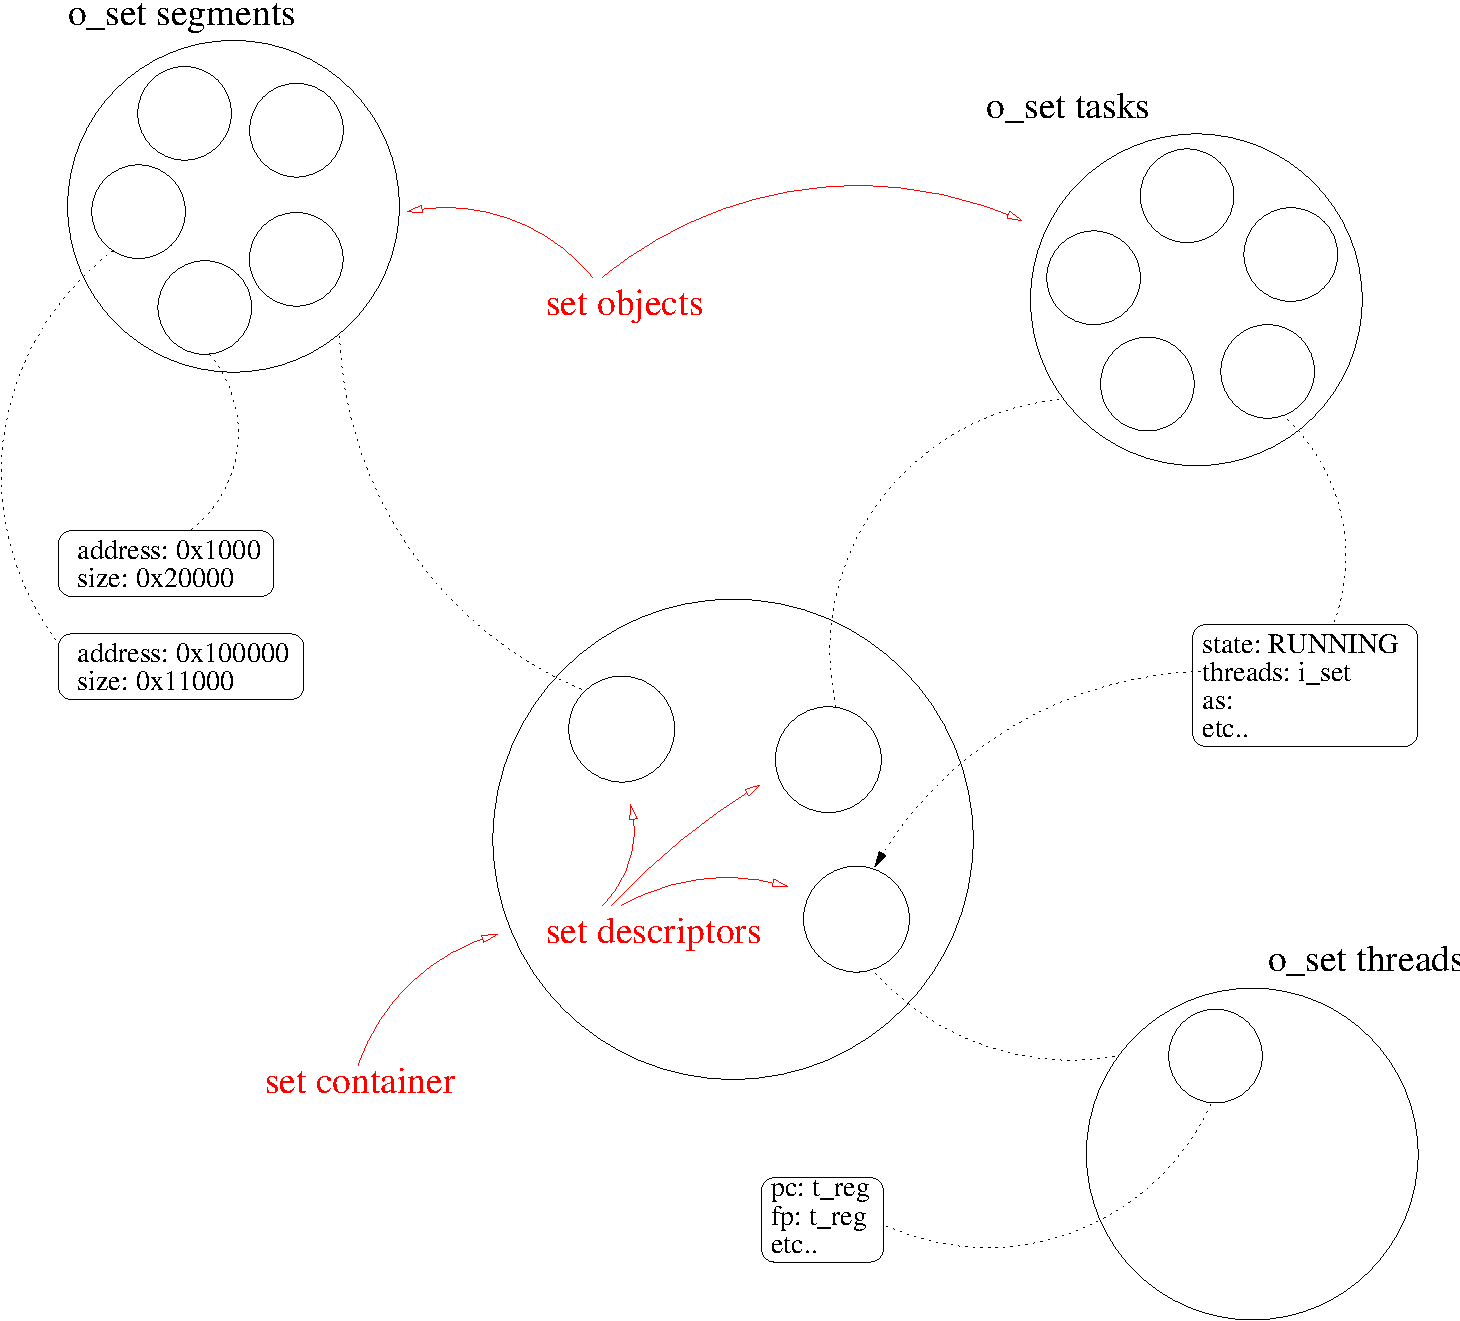
\includegraphics[scale=0.5]{figures/core_sets.pdf}
    \caption{Sets organization.}
    \label{figure:core_sets}
  \end{center}
\end{figure}

Note that the set manager is based on the \textit{malloc}() suite functions.
Indeed the set manager maintains a data structure containing the set
descriptors: the \textit{container}. Moreover some data structure
implementation require the \textit{malloc}() suite functions, the simplest
example being the array data structure which requires the \textit{realloc}()
function to be able to expand the data structure without effort.

Using this initial \textit{malloc}() function with its survival area,
the set manager is able to build sets for every kernel managers including
the segment manager, the address space manager, the region manager etc.

The set manager provides options to parameterize the set reservation.

The \textit{SET\_OPT\_CONTAINER} option is only used by the set manager
to build the very first set which then becomes the set container.

The \textit{SET\_OPT\_ALLOC} tells the set manager to always allocate
memory and to copy into this memory the content of the given object.
This option is very useful since the user never cares about allocating
memory. With this option, kaneton object stored in the set are automatically
freed when the set is released.

To tell the set manager to automatically free the objects stored without
setting the \textit{SET\_OPT\_ALLOC}, the \textit{SET\_OPT\_FREE} was
introduced. This option tells the set manager that the user will store
pre-allocated objects but the user wants them to be freed by the set
manager. This option is mutually exclusive with the
\textit{SET\_OPT\_ALLOC} option.

The \textit{SET\_OPT\_SORT} tells the set manager to always keep the set
sorted by identifiers.

The \textit{SET\_OPT\_ORGANISE} option is only used to re-organize the data
structure to keep it as simple as possible. This option may have no sens
with certain data structures.

%
% interface
%

\subsubsection{Interface}

\function{set\_type}{(i\_set \argument{id})}
	 {
	   This function just returns an error if the set corresponding
	   to \argument{id} is not of the type of the set implementation.
	 }

\function{set\_show}{(i\_set \argument{id})}
	 {
	   This function displays the entire set state of the set object
	   \argument{id}.
	 }

\function{set\_dump}{(void)}
	 {
	   This function displays all the set objects of the set manager.
	 }

\function{set\_size}{(i\_set \argument{id},
                      t\_setsz \argument{size})}
	 {
	   This function returns in \argument{size} the number of elements
	   of the set.
	 }

\function{set\_head}{(i\_set \argument{id},
                      t\_iterator* \argument{iterator})}
	 {
	   This function returns an iterator on the first element
	   of the set \argument{id}.
	 }

\function{set\_tail}{(i\_set \argument{id},
                      t\_iterator* \argument{iterator})}
	 {
	   This function returns an iterator on the last element of
	   the set \argument{id}.
	 }

\function{set\_previous}{(i\_set \argument{id},
                          t\_iterator \argument{current},
                          t\_iterator* \argument{previous})}
	 {
	   This function returns an iterator on the previous element
	   of the set.
	 }

\function{set\_next}{(i\_set \argument{id},
                      t\_iterator \argument{current},
                      t\_iterator* \argument{previous})}
	 {
	   This function returns an iterator on the next element
	   of the set.
	 }

\function{set\_insert}{(i\_set \argument{id},
                        void* \argument{data})}
	 {
	   This function inserts an object at the head of the set
	   \argument{id}.
	 }

\function{set\_append}{(i\_set \argument{id},
                        void* \argument{data})}
	 {
	   This function inserts an object at the tail of the set
	   \argument{id}.
	 }

\function{set\_before}{(i\_set \argument{id},
                        t\_iterator \argument{iterator},
                        void* \argument{data})}
	 {
	   This function inserts an object before the one specified
	   by the iterator.
	 }

\function{set\_after}{(i\_set \argument{id},
                       t\_iterator \argument{iterator},
                       void* \argument{data})}
	 {
	   This function inserts an object after the one specified
	   by the iterator.
	 }

\function{set\_add}{(i\_set \argument{id},
                     void* \argument{data})}
	 {
	   This function adds a data object in the set \argument{id}.
	 }

\function{set\_remove}{(i\_set \argument{id},
                        t\_id \argument{i})}
	 {
	   This function removes an object identified by \argument{i}
	   from the set \argument{id}.
	 }

\function{set\_delete}{(i\_set \argument{id},
                        t\_iterator \argument{iterator})}
	 {
	   This function deletes the object corresponding to the iterator.
	 }

\function{set\_flush}{(i\_set \argument{id})}
	 {
	   This function removes every object stored in the set
	   \argument{id}.
	 }

\function{set\_locate}{(i\_set \argument{id},
                        t\_id \argument{i},
                        t\_iterator* \argument{iterator})}
	 {
	   This function returns an iterator on the element corresponding
	   to the identifier \argument{i} of the set \argument{id}.
	 }

\function{set\_object}{(i\_set \argument{id},
                        t\_iterator \argument{iterator},
                        void** \argument{data})}
	 {
	   This function returns the data object corresponding to
	   the iterator.
	 }

\function{set\_push}{(i\_set \argument{id},
                      void* \argument{data})}
	 {
	   This function adds an object to a FIFO or LIFO structure.
	 }

\function{set\_pop}{(i\_set \argument{id})}
	 {
	   This function removes the next object of a FIFO or LIFO structure.
	 }

\function{set\_pick}{(i\_set \argument{id},
                      void** \argument{data})}
	 {
	   This function returns the next object of a FIFO or LIFO structure
	   without deleting it.
	 }

\function{set\_reserve}{(\argument{type},
                         t\_opts \argument{opts},
                         t\_size \argument{datasz},
                         i\_set* \argument{id})}
	 {
	   This function reserves a set object of type \argument{type}
	   with options \argument{opts} which will contain object of
	   \argument{datasz} size.

	   The reserved set object's identifier is returned in
	   \argument{id}.
	 }

\function{set\_release}{(i\_set \argument{id})}
	 {
	   This function releases the set \argument{id}.
	 }

\function{set\_initialize}{(void)}
	 {
	   This function initializes the set manager.
	 }

\function{set\_clean}{(void)}
	 {
	   This function cleans the set manager.
	 }

You can notice that some operations does not make sense on some data
structures. For example, \textit{set\_push}() or \textit{set\_pop}()
will never be used on arrays or lists, but only on stacks or pipes.

In these cases, the function must be implemented but will only return
an error.

Most widely, some operations have no sense with some options. Inserting
at the beginning of a sorted array must produce an error since it can
cancel the sorting property.

It is important to understand that a set implementation can specify
its own interface. Therefore, for example, the \textit{set\_reserve}()
function could have fifteen arguments for the stack implementation.

To better understand the implementations, take a look at the set
manager directory \textit{kaneton/core/set/} and its header file
\textit{kaneton/include/core/set.h}.

%
% stats manager
%

\section{stats manager}

The \textbf{stats manager} was introduced to perform runtime statistics on
the kaneton managers.

The kaneton object managed by the stats manager is the stats object
\textit{o\_stats} identified by a unique stats identifier \textit{i\_stats}.

Indeed, if enabled, every time a core function is called in a kaneton
manager, the stats manager is notified about that and then updates its
internal data structure.

Then, it is possible to perform statistics on the whole kaneton microkernel
and then to notice what are the most used managers and more precisly which
functions are widely called.

Note that the stats manager keeps track of the statistics via an internal
data structure. The stats manager does not use the set manager to store
its statistics. Indeed, if the stats manager used the set manager, it
would not be able to perform statistics on the set manager. In addition,
the set manager seems to be the most used manager so statistics must be
performed on it.

For this reason, the stats manager uses a specific data structure.

%
% interface
%

\subsubsection{Interface}

\function{stats\_show}{(i\_stats \argument{id})}
	 {
	   This function displays information about a stats object.
	 }

\function{stats\_dump}{(void)}
	 {
	   This function displays information on every stats object.
	 }

\function{stats\_begin}{(i\_stats \argument{id},
                         char* \argument{function})}
	 {
	   This function announces a new call of the function
	   \argument{function} in the stats object \argument{id}.
	 }

\function{stats\_end}{(i\_stats \argument{id},
                       char* \argument{function},
                       t\_error \argument{error})}
	 {
	   This function announces the end of a function call with the
	   return value \argument{error}.
	 }

\function{stats\_reserve}{(char* \argument{name},
                           i\_stats* \argument{id})}
	 {
	   This function reserves a stats object given a name \argument{name}.
	 }

\function{stats\_release}{(i\_stats \argument{id})}
	 {
	   This function releases a stats object.
	 }

\function{stats\_initialize}{(void)}
	 {
	   This function initializes the stats manager.
	 }

\function{stats\_clean}{(void)}
	 {
	   This function cleans the stats manager.
	 }

%
% as manager
%

\section{as manager}

The \textbf{address space manager} or \textbf{as manager} just manages
the address spaces objects.

An \textbf{address space object} or \textbf{as object} \textit{o\_as}
is an abstraction describing the addressable memory. The as objects
are identified by an address space identifier \textit{i\_as}.

An address space object is composed of a set of segments and a set of regions.

The set of segments describes the physical memory that belongs to this
address space while the set of regions describes the virtual memory
used to access the physical one.

It is important to understand that the set of segments holds segment
identifiers while the set of regions holds region objects.

%
% interface
%

\subsubsection{Interface}

\function{as\_show}{(i\_as \argument{id})}
	 {
	   This function shows a precise address space displaying
	   information on it.
	 }

\function{as\_dump}{(void)}
	 {
	   This function shows all the address space objects managed by
	   the address space manager.
	 }

\function{as\_give}{(i\_task \argument{task},
                     i\_as \argument{id})}
	 {
	   This function gives the address space \argument{id} to the
	   task object \argument{task}.
	 }

\function{as\_vaddr}{(i\_as \argument{id},
                      t\_paddr \argument{physical},
                      t\_vaddr* \argument{virtual})}
	 {
	   This function translates a physical address into its virtual
	   address.
	 }

\function{as\_paddr}{(i\_as \argument{id},
                      t\_vaddr \argument{virtual},
                      t\_paddr* \argument{physical})}
	 {
	   This function translates a virtual address into its physical
	   address.
	 }

\function{as\_clone}{(i\_task \argument{task},
                      i\_as \argument{old},
                      i\_as* \argument{new})}
	 {
	   This function clones an address space taking care of cloning
	   everything necessary: segments, regions etc.
	 }

\function{as\_reserve}{(i\_task \argument{task},
                        i\_as* \argument{id})}
	 {
	   This function reserves an address space object for the
	   task \argument{task} object.

	   The reserved address space object's identifier is returned
	   in \argument{id}.
	 }

\function{as\_release}{(i\_as \argument{id})}
	 {
	   This function just releases the address space \argument{id}.
	 }

\function{as\_get}{(i\_as \argument{id},
                    o\_as** \argument{o})}
	 {
	   This function should only be used by the as manager, the segment
	   manager and the region manager.

	   This function just returns the address space object
	   corresponding to the address space identifier \argument{id}.
	 }

\function{as\_initialize}{(void)}
	 {
	   This function initializes the address space manager.
	 }

\function{as\_clean}{(void)}
	 {
	   This function cleans the address space manager.
	 }

%
% segment manager
%

\section{segment manager}

The \textbf{segment manager} manages physical memory.

Its goals is to reserve and release physical memory areas, merge or split
allocated areas and finally to read or write directly into physical memory.

The kaneton object managed by the segment manager is the segment object.

A \textbf{segment object} \textit{o\_segment} describes an area of reserved
physical memory. A segment object has some properties like the base
address, the size, the permissions etc. and is identified by a
segment identifier \textit{i\_segment}.

In the current kaneton microkernel reference implementation, the
segment object's identifier is set from the segment object's base
address. Therefore, it is so easy to retrieve segment object from
the base address. Moreover, physical address are of course unique
so the segment objects can be stored in a set object without effort.

\function{segment\_show}{(i\_segment \argument{id})}
	 {
	   This function displays information on the specified segment
	   \argument{id}.
	 }

\function{segment\_dump}{(void)}
	 {
	   This function displays all segments of the set of segments.
	 }

\function{segment\_clone}{(i\_as \argument{as},
                           i\_segment \argument{old},
                           i\_segment* \argument{new})}
	 {
	   This function clones a segment which will then belong to
	   the address space object \argument{as}.

	   Cloning a segment means reserving a new segment with the
	   exact same properties. Then the content is also copied.
	 }

\function{segment\_inject}{(i\_as \argument{as},
                            o\_segment* \argument{o})}
	 {
	   This function injects a pre-allocated segment in the set of
	   segments.
	 }

\function{segment\_give}{(i\_as \argument{as},
                          i\_segment \argument{id})}
	 {
	   This function gives a segment from one address space to another.
	 }

\function{segment\_resize}{(i\_segment \argument{old},
                            t\_psize \argument{size},
                            i\_segment* \argument{new})}
	 {
	   This function resizes the segment \argument{old} to the
	   size \argument{size}.

	   The new segment, which can be the same, is returned in
	   \argument{new}.
	 }

\function{segment\_split}{(i\_segment \argument{id},
                           t\_psize \argument{size},
                           i\_segment* \argument{left},
                           i\_segment* \argument{rigth})}
	 {
	   This function splits the segment \argument{id} into two segments.

	   The size \argument{size} specifies the size of the new left segment.
	 }

\function{segment\_coalesce}{(i\_segment \argument{left},
                              i\_segment \argument{right},
                              i\_segment* \argument{id})}
	 {
	   This function merges two adjacent segments into a single
	   one \argument{id}.
	 }

\function{segment\_read}{(i\_segment \argument{id},
                          t\_paddr \argument{offset},
                          void* \argument{buffer},
                          t\_psize \argument{size})}
	 {
	   This function reads \argument{size} bytes at offset
	   \argument{offset} from the segment \argument{id}.
	 }

\function{segment\_write}{(i\_segment \argument{id},
                           t\_paddr \argument{offset},
                           const void* \argument{buffer},
                           t\_psize \argument{size})}
	 {
	   This function write the data of \argument{buffer} into the
	   segment \argument{id}.
	 }

\function{segment\_copy}{(i\_segment \argument{dst},
                          t\_paddr \argument{offd},
                          i\_segment \argument{src},
                          t\_paddr \argument{offs},
                          t\_psize \argument{size})}
	 {
	   This function copies data from the segment \argument{src} to
	   the segment \argument{dst}.
	 }

\function{segment\_reserve}{(i\_as \argument{as},
                             t\_psize \argument{size},
                             t\_perms \argument{perms},
                             i\_segment* \argument{id})}
	 {
	   This function reserves a segment with specified properties.
	 }

\function{segment\_release}{(i\_segment \argument{id})}
	 {
	   This function releases the segment \argument{id}.
	 }

\function{segment\_catch}{(i\_as \argument{as},
                           i\_segment \argument{id})}
	 {
	   This function is used to force a segment to be given to an address
	   space.

	   \notice{Catchable segments are reserved by the module service
	     for architecture specific servers. Catchable segments
	     are defined in the \argument{kaneton.conf} file.}
	 }

\function{segment\_perms}{(i\_segment \argument{id},
                           t\_perms \argument{perms})}
	 {
	   This function changes the permissions of the segment \argument{id}.
	 }

\function{segment\_type}{(i\_segment \argument{id},
                          t\_type \argument{type})}
	 {
	   This function changes the type of a segment.
	 }

\function{segment\_flush}{(i\_as \argument{as})}
	 {
	   This function removes every segment that belongs to the
	   address space \argument{as}.
	 }

\function{segment\_initialize}{(void)}
	 {
	   This function initializes the segment manager.
	 }

\function{segment\_clean}{(void)}
	 {
	   This function cleans the segment manager.
	 }

%
% region manager
%

\section{region manager}

The \textbf{region manager} manages mappings of segment called regions.

A \textbf{region object} \textit{o\_region} describes an area of virtual
memory mapping a segment part. Each region is identified by a unique region
identifier \textit{i\_region}.

As for segments, regions identifiers are set from the region base address.

\function{region\_show}{(i\_as \argument{as},
                         i\_region \argument{id})}
	 {
	   This function displays information on the specified region
	   \argument{id} of the address space object \argument{as}.
	 }

\function{region\_dump}{(i\_as \argument{as})}
	 {
	   This function displays all the regions of the address space
	   \argument{as}.
	 }

\function{region\_inject}{(i\_as \argument{as},
                           o\_region* \argument{o})}
	 {
	   This function injects a pre-allocated region in the set of
	   regions of the address space \argument{as}.
	 }

\function{region\_resize}{(i\_as \argument{as},
                           i\_region \argument{old},
                           t\_vsize \argument{size},
                           i\_region* \argument{new})}
	 {
	   This function resizes the region \argument{old} to the
	   size \argument{size}.

	   The new region, which can be the same, is returned in
	   \argument{new}.
	 }

\function{region\_reserve}{(i\_as \argument{as},
                            i\_segment \argument{segment},
                            t\_paddr \argument{offset},
                            \align{2.5cm}
                            t\_opts \argument{opts},
                            t\_vaddr \argument{address},
                            t\_vsize \argument{size},
                            i\_region* \argument{id})}
	 {
	   This function reserves a region with specified properties.
	 }

\function{region\_release}{(i\_as \argument{as},
                            i\_region \argument{id})}
	 {
	   This function releases the region \argument{id} that belongs
	   to the address space object \argument{as}.
	 }

\function{region\_flush}{(i\_as \argument{as})}
	 {
	   This function removes every region that belongs to the
	   address space \argument{as}.
	 }

\function{region\_initialize}{(void)}
	 {
	   This function initializes the region manager.
	 }

\function{region\_clean}{(void)}
	 {
	   This function cleans the region manager.
	 }

%
% map manager
%

\section{map manager}

It is obvious the programmer does not want to care about segments and
regions. He does not want to know what it is and why these things were
designed like that.

The programmer just wants to allocate memory. To make things easier
to the programmer, a map manager was introduced.

The \textbf{map manager} is just an abstract layer over the segment
and region manager.

Indeed its main task is to allocate memory so to reserve a segment
and a region mapping it.

%
% interface
%

\subsubsection{Interface}

\function{map\_reserve}{(i\_as \argument{as},
                         t\_opts \argument{opts},
                         t\_vsize \argument{size},
                         t\_perms \argument{perms},
                         t\_vaddr* \argument{address})}
	 {
	   This function reserves a mapping between a segment and a region.
	   The segment will have the size \argument{size} with the permissions
	   \argument{perms} while the region will map the whole segment.

	   The virtual address is returned in \argument{address}.
	 }

\function{map\_release}{(i\_as \argument{as},
                         t\_vaddr \argument{address})}
	 {
	   This function releases a previously reserved map.
	 }

\function{map\_initialize}{(void)}
	 {
	   This function initializes the map manager.
	 }

\function{map\_clean}{(void)}
	 {
	   This function cleans the map manager.
	 }

%
% event manager
%

\section{event manager}

The \textbf{event manager} manages such event objects.

An \textbf{event object} \textit{o\_event} is an abstraction over the
well-known hardware and software interrupts. Each event object is
identified by a unique event identifier \textit{i\_event}.

The events are used to describe a behaviour and to associate an action
to them.

Then, every time an hardware or software interrupt is triggered, the
architecture dependent code will pass on the information to the core
which will perform the associate action.

The common actions are either to run a specific event handler or to
send an event message to a specific kaneton task.

%
% interface
%

\function{event\_show}{(i\_event \argument{id})}
	 {
	   This function displays information on an event object.
	 }

\function{event\_dump}{(void)}
	 {
	   This function displays information on all the event objects.
	 }

\function{event\_reserve}{(i\_event \argument{id},
                           e\_event\_type \argument{type},
                           u\_event\_handler \argument{handler},
			   t\_vaddr \argument{data})}
	 {
	   This function installs an event handler. The \argument{data}
	   value will be passed as an argument of the handler.

	   The handler \argument{handler} is a function pointer when
	   \argument{type} is EVENT\_FUNCTION or a task identifier when
	   \argument{type} is EVENT\_MESSAGE.
	 }

\function{event\_release}{(i\_event \argument{id})}
	 {
	   This function releases an event object.
	 }

\function{event\_get}{(i\_event \argument{id},
                       o\_event** \argument{o})}
	 {
	   This function returns in \argument{o} the event object
	   corresponding to \argument{id}.
	 }

\function{event\_initialize}{(void)}
	 {
	   This function initializes the event manager.
	 }

\function{event\_clean}{(void)}
	 {
	   This function cleans the event manager.
	 }

%
% timer manager
%

\section{timer manager}

The \textbf{timer manager} manages timer objects.

A \textbf{timer object} \textit{o\_timer} is a timed event that measures
relative time. Each timer object is identified by a unique timer identifier
\textit{i\_timer}.

%
% interface
%

\function{timer\_show}{(i\_timer \argument{id})}
	 {
	   This function displays information on a timer object.
	 }

\function{timer\_dump}{(void)}
	 {
	   This function displays information on all the timers.
	 }

\function{timer\_reserve}{(t\_type \argument{type},
			   u\_timer\_handler \argument{handler},
			   t\_vaddr \argument{data},
                           t\_uint32 \argument{delay},
                           t\_uint32 \argument{repeat},
                           i\_timer* \argument{id})}
	 {
	   This function reserves a timer which will expire in
	   \argument{delay} microseconds.

	   The \argument{repeat} argument specifies if the timer
	   must be re-inserted once expired.

	   The \argument{data} value will be passed as an argument
	   of the handler.

	   The handler \argument{handler} is a function pointer when
	   \argument{type} is EVENT\_FUNCTION or a task identifier when
	   \argument{type} is EVENT\_MESSAGE.
	 }

\function{timer\_release}{(i\_timer \argument{id})}
	 {
	   This function releases a timer object.
	 }

\function{timer\_delay}{(i\_timer \argument{id},
                         t\_uint32 \argument{delay})}
	 {
	   This function updates the delay.
	 }

\function{timer\_repeat}{(i\_timer \argument{id},
                          t\_uint32 \argument{repeat})}
	 {
	   This function updates the repeat property.
	 }

\function{timer\_get}{(i\_timer \argument{id},
                       o\_timer** \argument{o})}
	 {
	   This function returns in \argument{o} the timer object
	   corresponding to \argument{id}.
	 }

\function{timer\_initialize}{(void)}
	 {
	   This function initializes the timer manager.
	 }

\function{timer\_clean}{(void)}
	 {
	   This function cleans the timer manager.
	 }

%
% task manager
%

\section{task manager}

The \textbf{task manager} provides a complete interface for the task
objects manipulation.

A \textbf{task object} \textit{o\_task} describes a complete execution
entity. Nevertheless, a task object is never scheduled since a task
is not an active entity.

A task is composed of an address space \textit{o\_as} and threads
\textit{o\_thread}.

Be careful, a task in the kaneton terms is different from a \textit{process}
in the UNIX{\copyright} terms. Indeed, a \textit{process} has only one
thread while kaneton tasks can have multiple ones. Nevertheless, the
term \textit{process} is sometimes used to describe a kaneton task.

Each task is identified by a unique task identifier \textit{i\_task}.

The task manager uses an internal nomenclature we will now detail.

The \textbf{class} \textit{t\_class} describes the task's rights on the
system. The different classes are \textit{TASK\_CLASS\_CORE},
\textit{TASK\_CLASS\_DRIVER}, \textit{TASK\_CLASS\_SERVICE} and
\textit{TASK\_CLASS\_PROGRAM}.

So a kaneton \textit{service} is in fact a task with a class
\textit{TASK\_CLASS\_SERVICE} and so on for the \textit{core},
\textit{drivers} and \textit{programs}.

These classes permit to give certain tasks, for example, the permission
to interact with hardware devices.

Moreover, this classification permit to build a tasks hierarchy.
Therefore, a task will be authorized to call another task only if
greater or equal privileged.

\notice{This calls hierarchy must be validated.}

The \textbf{behaviour} \textit{t\_behav} describes a priority
interval, each task being able to evolve in it by itself. The different
behaviors are \textit{TASK\_BEHAV\_CORE}, \textit{TASK\_BEHAV\_REALTIME},
\textit{TASK\_BEHAV\_INTERACTIVE}, \textit{TASK\_BEHAV\_TIMESHARING}
and \textit{TASK\_BEHAV\_BACKGROUND}.

The \textbf{priority} \textit{t\_prior} specify the current task
priority. Then, a task can updates its priority while this new priority
still is in the behaviour priority interval.

%
% interface
%

\subsubsection{Interface}

\function{task\_show}{(i\_task \argument{id})}
	 {
	   This function displays information on the task \argument{id}.
	 }

\function{task\_dump}{(void)}
	 {
	   This function displays information on every task.
	 }

\function{task\_clone}{(i\_task \argument{old},
                        i\_task* \argument{new})}
	 {
	   This function clones a task.

	   This function must take care of cloning everything necessary
	   including the address space and the threads.
	 }

\function{task\_reserve}{(t\_class \argument{class},
                          t\_behav \argument{behav},
                          t\_prior \argument{prior},
                          i\_task* \argument{id})}
	 {
	   This function reserves a task object with the given
	   properties: \argument{class}, \argument{behav} and
	   \argument{prior}.

	   Note that once reserved, the task is marked as stopped.
	 }

\function{task\_release}{(i\_task \argument{id})}
	 {
	   This function releases the task object \argument{id}.
	 }

\function{task\_priority}{(i\_task \argument{id},
                           t\_prior \argument{prior})}
	 {
	   This function updates the task's priority to \argument{prior}.
	 }

\function{task\_run}{(i\_task \argument{id})}
	 {
	   This function marks the task as runnable.
	 }

\function{task\_stop}{(i\_task \argument{id})}
	 {
	   This function stops the task \argument{id}.
	 }

\function{task\_exit}{(i\_task \argument{id})}
	 {
	   This function kills the task \argument{id} which is forced to
	   exit. In this case, the threads are stopped and the task becomes
	   a \textit{zombie}.
	 }

\function{task\_wait}{(i\_task \argument{id},
                       t\_opts \argument{opts},
                       t\_wait* \argument{wait})}
	 {
	   This function waits for state change in one or more tasks
	   depending on the options \argument{opts}.

	   The flags of \argument{opts} specify the state to wait for:
	   \textit{WAIT\_DEATH}, \textit{WAIT\_START},
	   \textit{WAIT\_STOP} and \textit{WAIT\_ALL}.

	   Moreover, other flags are used to precise the tasks to wait for:
	   \textit{WAIT\_ID} for a precise task \argument{id} or
	   \textit{WAIT\_CHILDREN} for any children.

	   Finally, another flag \textit{WAIT\_NOHANG} can be used
	   to make the function non-blocking if no task's state has changed.

	   \notice{All these features are not implemented yet.}

	   \notice{We could probably extend the waiting states to more
	     exotic ones like WAIT\_IO etc.}
	 }

\function{task\_get}{(i\_task \argument{id},
                      o\_task** \argument{o})}
	 {
	   This function returns in \argument{o} the task object corresponding
	   to \argument{id}.
	 }

\function{task\_initialize}{(void)}
	 {
	   This function initializes the task manager.
	 }

\function{task\_clean}{(void)}
	 {
	   This function cleans the task manager.
	 }

%
% thread manager
%

\section{thread manager}

The \textbf{thread manager} manages the real active execution context
called threads.

A \textbf{thread object} is an active entity which describes the
current state of an execution context including the \textit{program counter},
the \textit{stack pointer} etc.

Indeed, a thread is composed of a current \textit{program counter} which
keeps the next instruction address to execute and the \textit{stack pointer}
which keeps the stack address. With these two characteristics, a thread
can be described.

Needless to say, some additional architecture-dependent properties are
required to fully describe a thread context.

Like the tasks, each thread has its own priority meaning that each thread
can parameterize its scheduling priority.

The threads' priorities must be contained in the interval $[10, 250[$, the
macro \textit{THREAD\_PRIOR} representing the default priority.

%
% interface
%

\subsubsection{Interface}

\function{thread\_show}{(i\_thread \argument{id})}
	 {
	   This function displays information on the thread \argument{id}.
	 }

\function{thread\_dump}{(void)}
	 {
	   This function displays information on all the threads.
	 }

\function{thread\_give}{(i\_task \argument{task},
                         i\_thread \argument{id})}
	 {
	   This function gives the thread object \argument{id} to the
	   task \argument{task}.
	 }

\function{thread\_clone}{(i\_task \argument{task},
                          i\_thread \argument{old},
                          i\_thread* \argument{new})}
	 {
	   This function clones the task \argument{old} into a new one
	   \argument{new}.

	   This new thread, having the exact same properties as \argument{old},
	   will be held by the task \argument{task}.
	 }

\function{thread\_reserve}{(i\_task \argument{task},
                            t\_prior \argument{prior},
                            i\_thread* \argument{id})}
	 {
	   This function reserves a thread for the task \argument{task}
	   given the default thread priority \argument{prior}.

	   Note that once reserved, the thread is marked as stopped.
	 }

\function{thread\_release}{(i\_thread \argument{id})}
	 {
	   This function releases the thread object \argument{id}.
	 }

\function{thread\_priority}{(i\_thread \argument{id},
                             t\_prior \argument{prior})}
	 {
	   This function updates the current thread priority
	   to \argument{prior}.
	 }

\function{thread\_run}{(i\_thread \argument{id})}
	 {
	   This function marks the thread object \argument{id}
	   as runnable.
	 }

\function{thread\_stop}{(i\_thread \argument{id})}
	 {
	   This function stops the thread object \argument{id}.
	 }

\function{thread\_exit}{(i\_thread \argument{id})}
	 {
	   This function kills the thread \argument{id} forcing it to
	   exit.

	   Therefore, if all the threads of the same task have exited, the
	   task must exit too via the \textbf{task\_exit}() function.
	 }

\function{thread\_wait}{(i\_thread \argument{id},
                         t\_opts \argument{opts},
                         t\_wait* \argument{wait})}
	 {
	   This function acts like the function \textbf{task\_wait}().

	   This function waits for the thread's state to change depending on
	   the options \argument{opts}.
	 }

\function{thread\_get}{(i\_thread \argument{id},
                        o\_thread** \argument{o})}
	 {
	   This function returns in \argument{o} the thread object
	   corresponding to \argument{id}.
	 }

\function{thread\_flush}{(i\_task \argument{task})}
	 {
	   This function removes every thread that belongs to the
	   task object \argument{task}.
	 }

\function{thread\_stack}{(i\_thread \argument{id},
                          t\_vsize \argument{size})}
	 {
	   This function allocates a stack of \argument{size} bytes
	   for the thread \argument{id}.
	 }

\function{thread\_load}{(i\_thread \argument{id},
                         t\_thread\_context \argument{context})}
	 {
	   This function loads a new execution context in the thread
	   object \argument{id}.

	   A thread execution context \textit{t\_thread\_context}
	   only contains the \textit{program counter} and the
	   \textit{stack pointer}.
	 }

\function{thread\_store}{(i\_thread \argument{id},
                          t\_thread\_context* \argument{context})}
	 {
	   This function stores in \argument{context} the current
	   thread execution context of the thread object \argument{id}.
	 }

\function{thread\_args}{(i\_thread \argument{id},
                         void* \argument{args},
                         t\_size \argument{size})}
	 {
	   This function installs the arguments of the thread \argument{id}
	   on its stack.

	   In other words, this function copies \argument{size} bytes
	   from \argument{args} on the thread's stack.

	   Note that this function was designed to fit the general case.
	   Indeed, the special case of the \textit{main}() function
	   with its arguments \textit{argc} and \textit{argv} is not
	   directly handled by this function.

	   A C library function must be used to pack command line
	   argument strings into a unique arguments array. Then the
	   \textbf{thread\_args}() function can be used to install
	   this array onto the stack.
	 }

\function{thread\_initialize}{(void)}
	 {
	   This function initializes the thread manager.
	 }

\function{thread\_clean}{(void)}
	 {
	   This function cleans the thread manager.
	 }

%
% scheduler
%

\section{scheduler}

The \textbf{scheduler}'s role is to schedule the threads' execution
based on some properties like the tasks' behaviors, the tasks' priorities
and the threads' priorities.

Be careful, the scheduler schedules the threads which are the active
execution entities and not the tasks.

Current implementation of the scheduler uses a multilevel feedback
queues algorithm. The scheduler, in conjunction with the \textbf{cpu
manager}, supports multiple processors.

%
% interface
%

\subsubsection{Interface}

\function{scheduler\_quantum}{(t\_quantum \argument{quantum})}
	 {
	   This function sets the scheduler quantum to \argument{quantum}.
	 }

\function{scheduler\_yield}{(i\_cpu \argument{cpuid})}
	 {
	   This function permits the current task to relinquish
	   the processor \argument{cpuid} voluntarily.
	 }

\function{scheduler\_add}{(i\_thread \argument{thread})}
	 {
	   This function adds a runnable thread to the scheduler.
	 }

\function{scheduler\_remove}{(i\_thread \argument{thread})}
	 {
	   This function remove a thread from the scheduler.
	 }

\function{scheduler\_update}{(i\_thread \argument{thread})}
	 {
	   This function asks the scheduler to update the thread
	   \argument{thread} in its internal data structures since
	   for example the thread's priority just changed.
	 }

\function{scheduler\_current}{(i\_thread* \argument{thread})}
	 {
	   This function returns in \argument{thread} the identifier
	   of the thread currently executed on the current processor.
	 }

\function{scheduler\_switch}{(void)}
	 {
	   This function just schedules a new elected thread.
	 }

\function{scheduler\_initialize}{(void)}
	 {
	   This function initializes the scheduler.
	 }

\function{scheduler\_clean}{(void)}
	 {
	   This function cleans the scheduler.
	 }

%
% scheduler
%

\section{cpu manager}

The \textbf{cpu manager} provides all mecanisms to support
symmetrical multiprocessor platforms.

The interface of this manager provides functions to assign a processor
to a newly created task, to migrate a task from one processor to
another and to perform load-balancing.

A \textbf{cpu object} contains information dealing about a
microprocessor's load weight and efficiency. These statistics are
updated by the scheduler, which reports the current activity of each
processors (like the effective timeslice of a thread on a given
microprocessor.

%
% interface
%

\subsubsection{Interface}

\function{cpu\_show}{(i\_cpu \argument{id})}
	 {
	   This function displays information on the processor \argument{id}.
	 }

\function{cpu\_dump}{(void)}
	 {
	   This function displays information on all the active
	   microprocessors.
	 }

\function{cpu\_current}{(i\_cpu* \argument{id})}
	 {
	   This function sets \argument{id} to the identifier of the
	   microprocessor on which the kernel is currently running.
	 }

\function{cpu\_select}{(i\_cpu* \argument{id})}
	 {
	   This function is called when a new task is created. It gives
	   the identifier of the microprocessor with the lowest load.
	 }

\function{cpu\_stats}{(i\_cpu \argument{id},
                       t\_timeslice \argument{time})}
	 {
	   This function updates statistics for the processor \argument{id}.

	   \notice{This function will be extended to provide more
	   precise statistics.}
	 }

\function{cpu\_balance}{(void)}
	 {
	   This function -- called periodically -- performs a
	   load-balancing on all processors.
	 }

\function{cpu\_migrate}{(i\_task \argument{tskid},
                         i\_cpu \argument{destination})}
	 {
	   This function migrates the task \argument{tskid} to the
	   processor \argument{destination}.
	 }

\function{cpu\_get}{(i\_cpu \argument{id},
                     o\_cpu** \argument{o})}
	 {
	   This function get the object corresponding to the processor
	   \argument{id}.
	 }

\function{cpu\_initialize}{(void)}
	 {
	   This function initializes the cpu manager.
	 }

\function{cpu\_clean}{(void)}
	 {
	   This function cleans the cpu manager.
	 }

\notice{The cpu manager is not yet finished. For the moment, it only
supports a single microprocessor.}

%
% message manager
%

\section{message manager}

The \textbf{message manager} provides a complete interface to send and
receive messages in many different ways.

The kaneton message interface directly comes from standards in parallel
and distributed programming.

The message manager provides blocking and non-blocking functions,
synchronous and asynchronous messages etc.

A synchronous function is a function which does not permit the calling
task to execute instructions until the message is fully copied to the
destination buffer.

In a performance perpective, in Kaneton, kernel bufferization is avoided
as much as possible.

A blocking function is a function which does not return until the
action is totally performed. As a non-blocking function does not certify
that the action has been performed when the function returns, that is to
say we don't know if the given buffer has been entirely read/written. With
non-blocking functions, sending/receiving buffers are not securely accessible
until we are not assured that the message is copied somewhere. Functions
\textit{message\_wait}() and \textit{message\_status}() are provided for
this.

The messaging primitives are accessible from userspace through syscalls,
functions parameters are passed through CPU registers. Messages bound for
the kernel are directly redirected to the interface manager.

Each messages has a type which is associated with a message size. For each
tasks, used types must be registered.

\notice{The system calls corresponding to these functions do not take
the first argument, which is in all cases an \argument{i\_task}}

%
% interface
%

\subsubsection{Interface}

\function{message\_register}{(i\_task \argument{task},
			      t\_type \argument{type},
			      t\_vsize \argument{size})}
	 {
	   This function registers for the task \argument{task} the type
	   of message \argument{type} for which the maximum size is
	   \argument{size} bytes long.
	 }

\function{message\_send}{(i\_task \argument{task},
			  i\_node \argument{destination},
			  t\_type \argument{type},
			  t\_vaddr \argument{data},
			  t\_vsize \argument{size})}
	 {
	   This blocking function performs an asynchronous send of the
	   message of registered type \argument{type} located at
	   \argument{data} of size \argument{size} to the node
	   \argument{destination} in the distributed system.
	 }

\function{message\_transmit}{(i\_task \argument{task},
			      i\_node \argument{destination},
			      t\_type \argument{type},
			      t\_vaddr \argument{data},
			      t\_vsize \argument{size})}
	 {
	   This blocking function performs a synchronous send of the
	   message of registered type \argument{type} located at
	   \argument{data} of size \argument{size} to the node
	   \argument{destination} in the distributed system.
	 }

\function{message\_throw}{(i\_task \argument{task},
			   i\_node \argument{destination},
			   t\_type \argument{type},
			   t\_vaddr \argument{data},
			   t\_vsize \argument{size},
			   t\_message\_request* \argument{request})}
	 {
	   This blocking function performs an asynchronous send of the
	   message of registered type \argument{type} located at
	   \argument{data} of size \argument{size} to the node
	   \argument{destination} in the distributed system.

	   The \argument{request} argument will be needed after the call
	   to control the completeness of the operation.

	   \notice{On uniprocessor systems, this function is simply an
	     alias to \argument{message\_send()}}
	 }

\function{message\_receive}{(i\_task \argument{task},
			     t\_type \argument{type},
			     t\_vaddr \argument{data},
			     i\_node* \argument{sender})}
	 {
	   This blocking function waits (stop calling thread execution)
	   until a message of register type \argument{type} is received.
	   The message content is copied at address \argument{data} and
	   the sender is returned in \argument{sender}.
	 }

\function{message\_poll}{(i\_task \argument{task},
			  t\_type \argument{type},
			  t\_vaddr \argument{data},
			  i\_node* \argument{sender})}
	 {
	   This blocking function look for a message of register type
	   \argument{type} being received, and otherwise returns an error.
	   The message content is copied at address \argument{data} and
	   the sender is returned in \argument{sender}.
	 }

\function{message\_grab}{(i\_task \argument{task},
			  t\_type \argument{type},
			  t\_vaddr \argument{data},
			  i\_node* \argument{sender},
			  t\_message\_request* \argument{request})}
	 {
	   This non-blocking function receives a message of register
	   type \argument{type}.
	   The message content is copied at address \argument{data} and
	   the sender is returned in \argument{sender}.

	   The argument \argument{request} is later used to check the
	   status of the operation.

	   \notice{On uniprocessor systems, this function is simply an
	     alias to \argument{message\_receive()}}
	 }

\function{message\_wait}{(i\_task \argument{task},
			  t\_message\_request \argument{request})}
	 {
	   This function blocks the calling task until the message request
	   described by \argument{request} is fully completed.
	 }


\function{message\_state}{(i\_task \argument{task},
			   t\_message\_request \argument{request})}
	 {
	   This function returns whether the message request described
	   by \argument{request} is fully completed or not.
	 }

\function{message\_return}{(i\_thread \argument{thread},
			    t\_error \argument{code})}
	 {
	   This function sets the return value \argument{code} for a
	   blocked thread during a \argument{message\_transmit()} operation.

	   \notice{This function is used internally by the manager and
	     thus is not exported as a system call.}
	 }

\function{message\_return\_info}{(i\_thread \argument{thread},
				  t\_error \argument{code},
				  t\_vsize \argument{size},
				  i\_node \argument{sender})}
	 {
	   This function sets the return values \argument{code},
	   \argument{size} and \argument{sender} for a blocked thread
	   during a \argument{message\_receive()} operation.

	   \notice{This function is used internally by the manager and
	     thus is not exported as a system call.}
	 }

\begin{comment}


\end{comment}

%
% io manager
%

\section{io manager}

The \textbf{io manager} provides an interface to interact with
hardware through the microprocessor I/O ports or through memory mapped
I/O.

We use the term ``I/O port'', even if it refers to memory-mapped I/O
depending on the architecture.

The control of I/O ports access is implemented \textit{via} a couple
of functions that allow or deny one precise task from reading or
writing to a port. There is no way to deny a given operation (eg:
reading or writing).

The read and write operations are performed by the io manager
architecture dependent part.

%
% interface
%

\subsubsection{Interface}

\function{io\_grant}{(i\_port \argument{id},
                      i\_task \argument{task},
                      t\_uint8 \argument{width})}
	 {
	   This function grant \argument{task} for accessing
	   \argument{width} bytes of \argument{id} port both for
	   reading and writing.
	 }

\function{io\_deny}{(i\_port \argument{id},
                     i\_task \argument{task},
                     t\_uint8 \argument{width})}
	 {
	   This function deny \argument{task} for accessing
	   \argument{width} bytes of \argument{id} port both for
	   reading and writing.
	 }

\function{io\_read\_8}{(i\_task \argument{task},
                        i\_port \argument{id},
                        t\_uint8* \argument{data})}
	 {
	   This function reads a byte from \argument{id} port for
	   \argument{task}.
         }

\function{io\_read\_16}{(i\_task \argument{task},
                         i\_port \argument{id},
                         t\_uint16* \argument{data})}
	 {
	   This function reads a 16 bits word from \argument{id} port for
	   \argument{task}.
         }

\function{io\_read\_32}{(i\_task \argument{task},
                         i\_port \argument{id},
                         t\_uint32* \argument{data})}
	 {
	   This function reads a 32 bits word from \argument{id} port for
	   \argument{task}.
         }

\function{io\_read\_64}{(i\_task \argument{task},
                         i\_port \argument{id},
                         t\_uint64* \argument{data})}
	 {
	   This function reads a 64 bits word from \argument{id} port for
	   \argument{task}.
         }

\function{io\_write\_8}{(i\_task \argument{task},
                         i\_port \argument{id},
                         t\_uint8 \argument{data})}
	 {
	   This function write a byte to \argument{id} port for
	   \argument{task}.
         }

\function{io\_write\_16}{(i\_task \argument{task},
                          i\_port \argument{id},
                          t\_uint16 \argument{data})}
	 {
	   This function write a 16 bits word to \argument{id} port for
	   \argument{task}.
         }

\function{io\_write\_32}{(i\_task \argument{task},
                          i\_port \argument{id},
                          t\_uint32 \argument{data})}
	 {
	   This function write a 32 bits word to \argument{id} port for
	   \argument{task}.
         }

\function{io\_write\_64}{(i\_task \argument{task},
                          i\_port \argument{id},
                          t\_uint64 \argument{data})}
	 {
	   This function write a 64 bits word to \argument{id} port for
	   \argument{task}.
         }

\function{io\_initialize}{(void)}
	 {
	   This function initializes the io manager.
	 }

\function{io\_clean}{(void)}
	 {
	   This function cleans the io manager.
	 }

\notice{All read/write functions may not be implemented depending of
the architecture.}
